% !TeX spellcheck = ru_RU
\chapter{Выполнение лабораторной работы}

\section{Цель работы}

Лабораторная работа № 3 нацелена на знакомство с возможностями программы Microsoft Project по контролю за ходом реализации проекта.


\section{Краткое описание проекта}

Команда разработчиков из 16 человек занимается созданием карты города на основе собственного модуля отображения. Проект должен быть завершен в течение 6 месяцев. Бюджет проекта: 50 000 рублей.

\section{Общее задание по варианту}

Дата отчета~---~10 мая. Отметить как выполненные все работы, которые должны были завершиться на эту дату, кроме:
\begin{enumerate}
	\item 10 марта для задач по дизайну интерфейса (№4--6) купили специализированное ПО, стоимость которого составила 1200 руб. В результате фактические трудозатраты на выполнение этих задач увеличились на 10\% по каждой задаче;
	\item задача №13 фактически завершилась 30.03;
	\item задача №15 фактически выполнена на 70\%;
	\item с 4 апреля программисты №1 и №3 были отправлены в командировку на 2 недели. На это время рабочее время программистов №2 и №4 было увеличено до 10 часов/день, а их зарплата повышена на 20\%.
	\item с 30.04 уволился один из наборщиков данных;
	\item с 11 апреля на 5\% увеличилась стоимость аренды сервера.
\end{enumerate}

\section{Базовый план проекта}

На рисунках~\ref{fig:1}и~\ref{fig:2} представлены список задач и лист ресурсов соответственно, установленные в качестве базового плана, как показано на рисунке~\ref{fig:3}.

\begin{figure}[H]
	\centering
	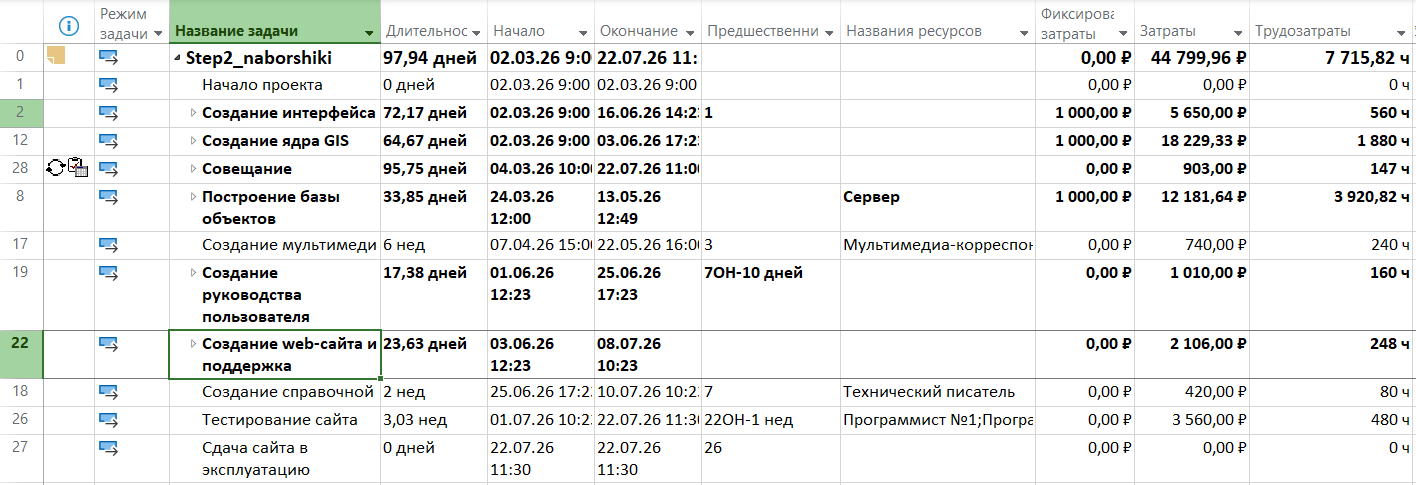
\includegraphics[width=\linewidth]{images/baseline.png}
	\caption{План работ и диаграмма Ганта сохраненные в качестве базового плана}
	\label{fig:1}
\end{figure}

\begin{figure}[H]
\centering
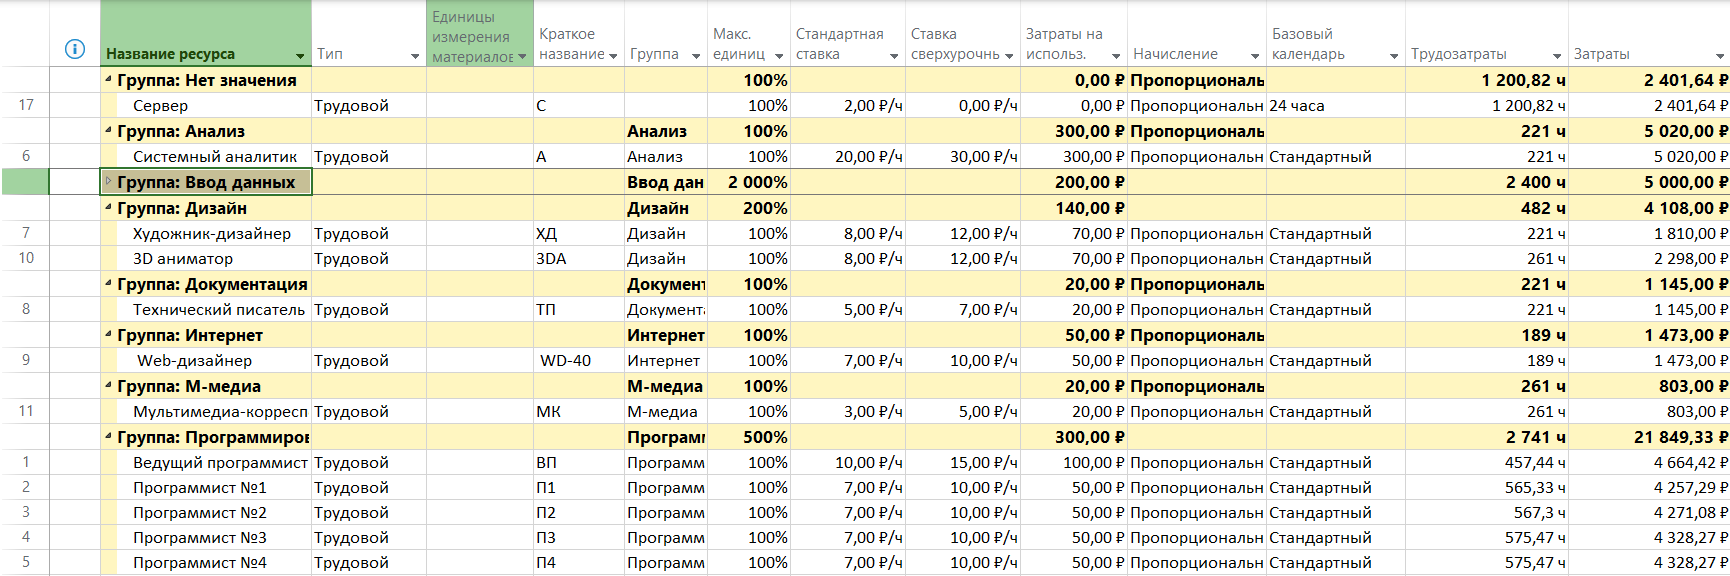
\includegraphics[width=\linewidth]{images/baseline_resurs.png}
\caption{Лист ресурсов сохраненный в качестве базового плана}
\label{fig:2}
\end{figure}

\begin{figure}[H]
\centering
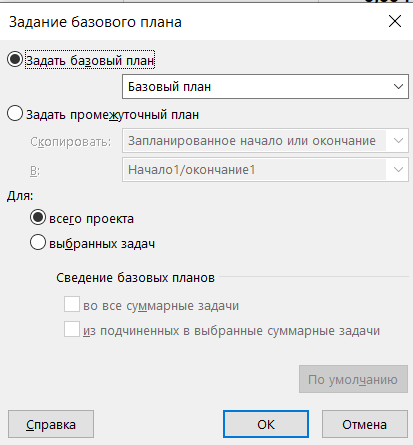
\includegraphics[width=0.5\linewidth]{images/save_baseline.png}
\caption{Сохранение базового плана проекта}
\label{fig:3}
\end{figure}

\section{Задание 1}

Затраты на закупку по вносятся как фиксированные затраты задачи №3 подзадачами которой, являются задачи №4--6. Трудозатраты по задачам №4--6 составили 132, 88, 132 часа соответственно. В результате изменения трудозатрат, возникли перегрузки, как показано на рисунке~\ref{fig:4}.

\begin{figure}[H]
	\centering
	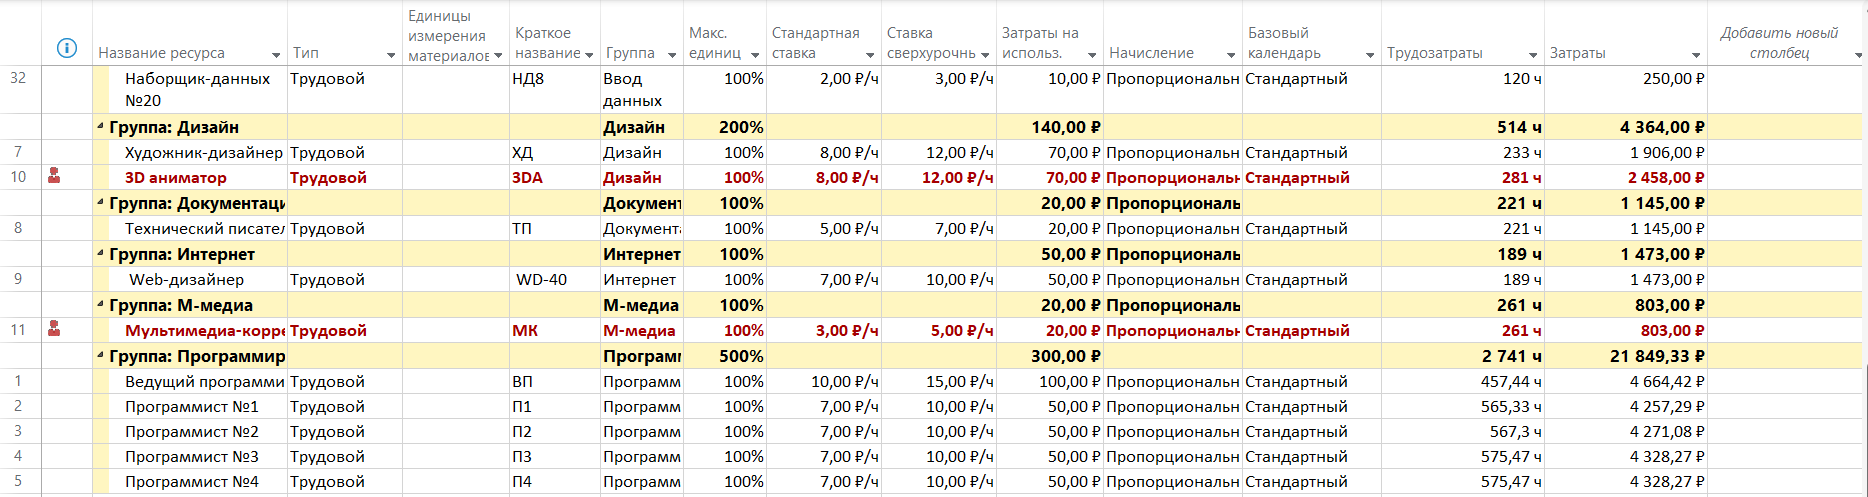
\includegraphics[width=\linewidth]{images/peregruz.png}
	\caption{Перегрузки ресурсов в результате увеличения трудозатрат по задачам №4--6}
	\label{fig:4}
\end{figure}

Для разрешения перегрузок, использовалось автоматическое выравнивание, что привело сдвигу срока завершения родительской задачи №3 на 3 дня, до 10.04 и увеличению затрат до 46 259,96 (+1460) рублей. При этом общие сроки проекта не изменились, так как данные задачи не лежат на критическом пути. Результат показан на рисунке~\ref{fig:5}.

\begin{figure}[H]
	\centering
	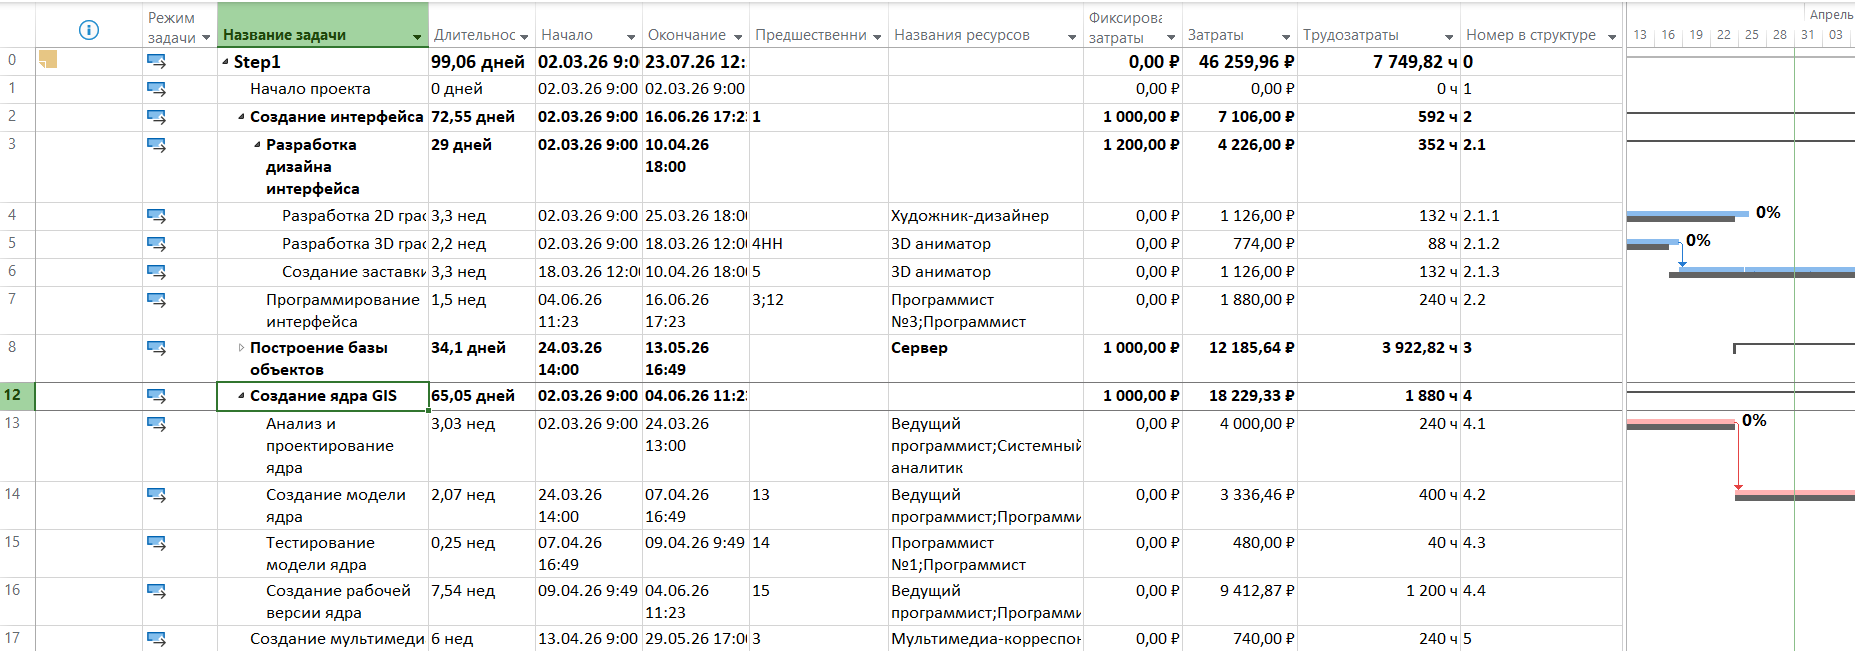
\includegraphics[width=\linewidth]{images/solve_peregruz_1_align_po_chasam.png}
	\caption{Результат разрешения перегрузки для ресурсов}
	\label{fig:5}
\end{figure}

\section{Задание 2}

Завершение задачи №13 было выставлено в меню <<Обновление задачи>> на 30.03~\ref{fig:6}. В результате изменения сроков завершения задачи возникли перегрузки, как показано на рисунке~\ref{fig:7}. После автоматического разрешения перегрузок, сроки проекта сдвинулись на 30.07, а бюджет увеличился до 46 775,88 (+515,92) рублей~\ref{fig:8}.

\begin{figure}[H]
	\centering
	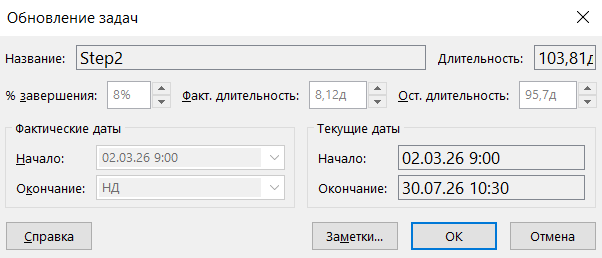
\includegraphics[width=\linewidth]{images/update_task.png}
	\caption{Обновление сроков задачи №13}
	\label{fig:6}
\end{figure}

\begin{figure}[H]
	\centering
	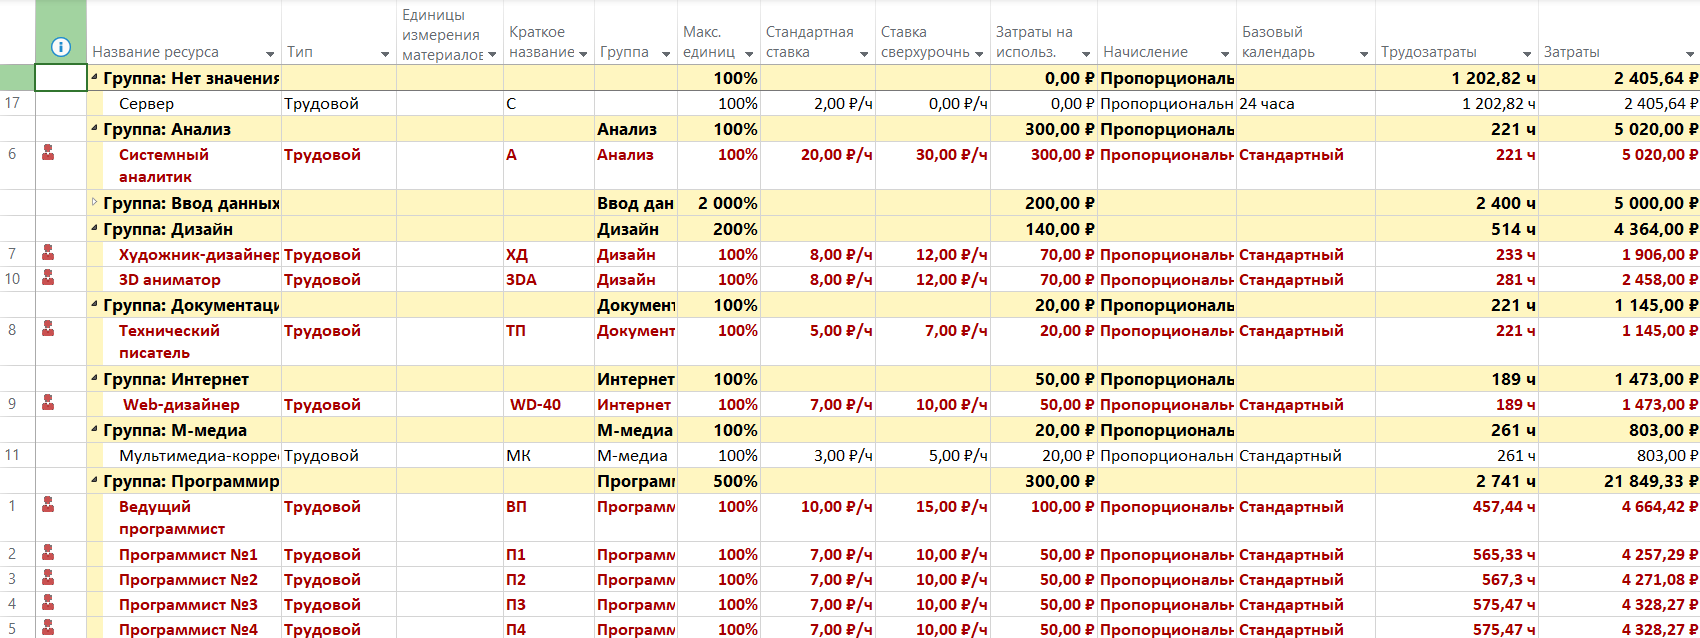
\includegraphics[width=\linewidth]{images/peregruz_2_after_change_srok_13_resurs.png}
	\caption{Перегрузка ресурсов в результате изменения сроков задачи №13}
	\label{fig:7}
\end{figure}

\begin{figure}[H]
	\centering
	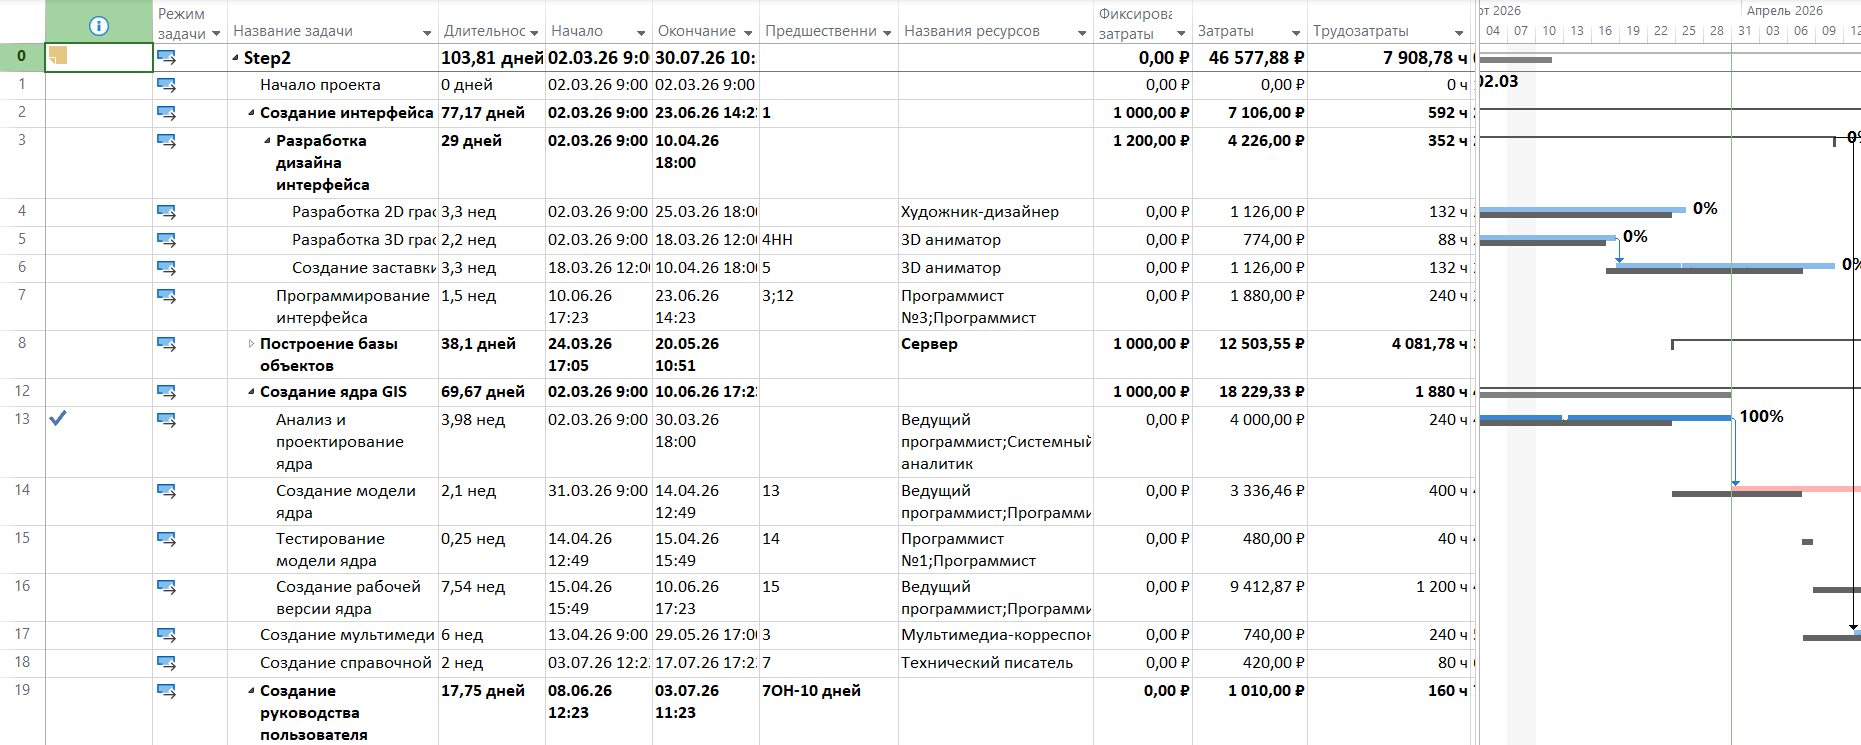
\includegraphics[width=\linewidth]{images/solve_peregruz_2_po_chasam.png}
	\caption{Результат разрешения перегрузки для ресурсов}
	\label{fig:8}
\end{figure}

\section{Задание 3}

Для установки фактического завершения задачи №15 использовалось меню <<Обновление задачи>>, как показано на рисунке~\ref{fig:9}.

\begin{figure}[H]
	\centering
	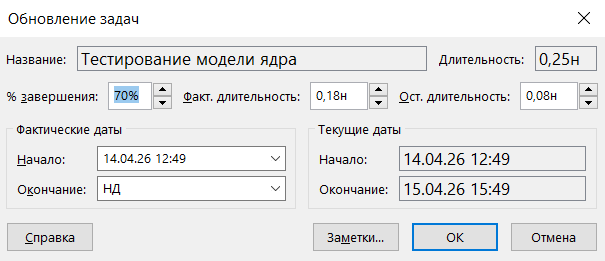
\includegraphics[width=\linewidth]{images/update_task_2.png}
	\caption{Установка значения фактического уровня выполнения задачи}
	\label{fig:9}
\end{figure}

Установка процента выполнения задачи не повлияла на сроки выполнения задачи и бюджет.

\section{Задание 4}

Для отображения информации об отправке программистов №1 и №3 в командировку, были изменены сведения об их доступности, как показано на рисунке~\ref{fig:10}. Установка сведений об увеличении длины рабочего дня и оплаты для программистов №2 и №4 представлена на рисунках~\ref{fig:11} и~\ref{fig:12} соответственно. В результате возникли перегрузки для программистов, как показано на рисунке~\ref{fig:13}. Для устранения перегрузки была опробована возможность изменить профиль загрузки, но автоматическое выравнивание оказалось эффективней. В результате автоматического выравнивания сроки проекта сдвинулись до 12.08, а затраты до 49 585,53 (+3007,65) рублей~\ref{fig:14}.

\begin{figure}[H]
	\centering
	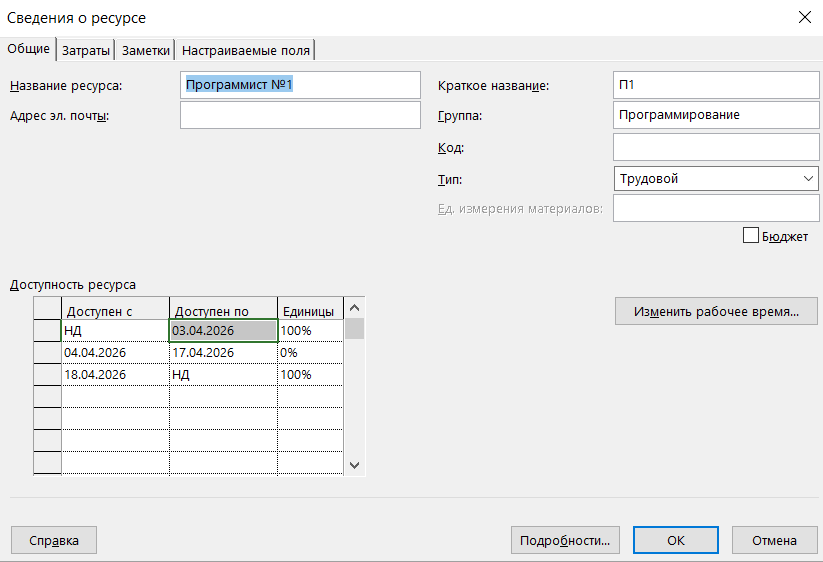
\includegraphics[width=0.7\linewidth]{images/komandirovka.png}
	\caption{Установка сведений о доступности программистов №1 и №3 на период командировки}
	\label{fig:10}
\end{figure}

\begin{figure}[H]
	\centering
	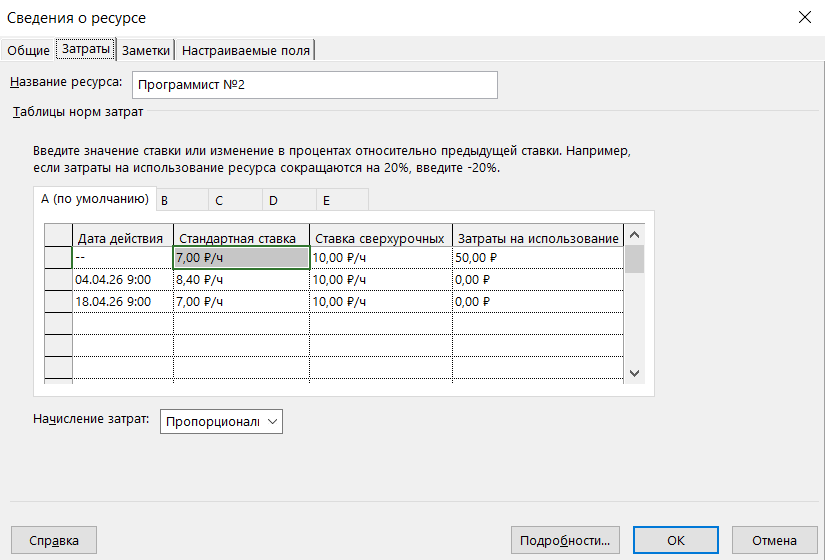
\includegraphics[width=0.7\linewidth]{images/babki.png}
	\caption{Установка сведений об увеличении оплаты для программистов №2 и №4}
	\label{fig:11}
\end{figure}

\begin{figure}[H]
	\centering
	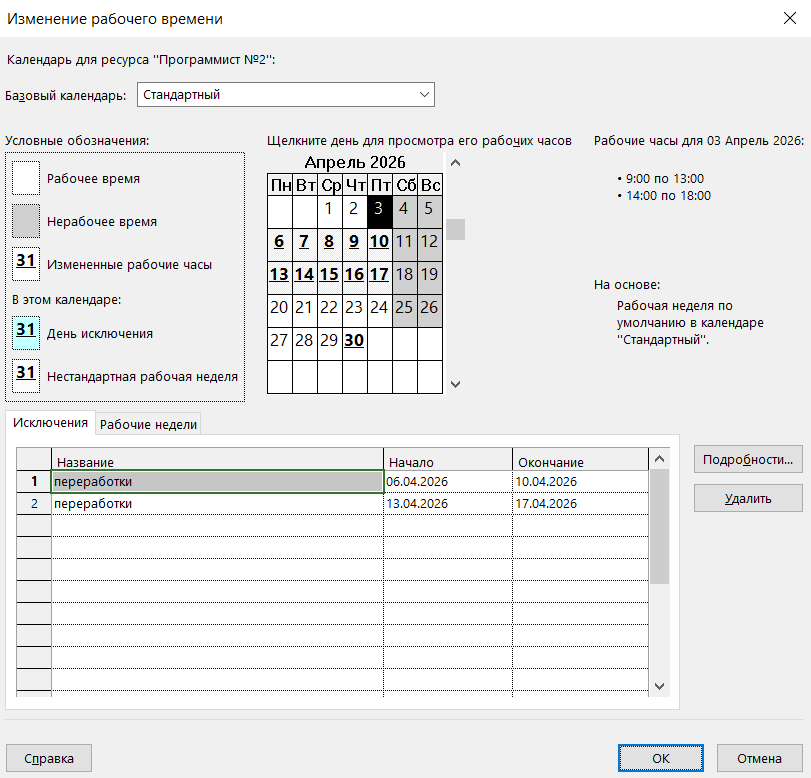
\includegraphics[width=0.7\linewidth]{images/pererabotka.png}
	\caption{Установка сведений об увеличенной длительности рабочего дня для программистов №2 и №4}
	\label{fig:12}
\end{figure}

\begin{figure}[H]
	\centering
	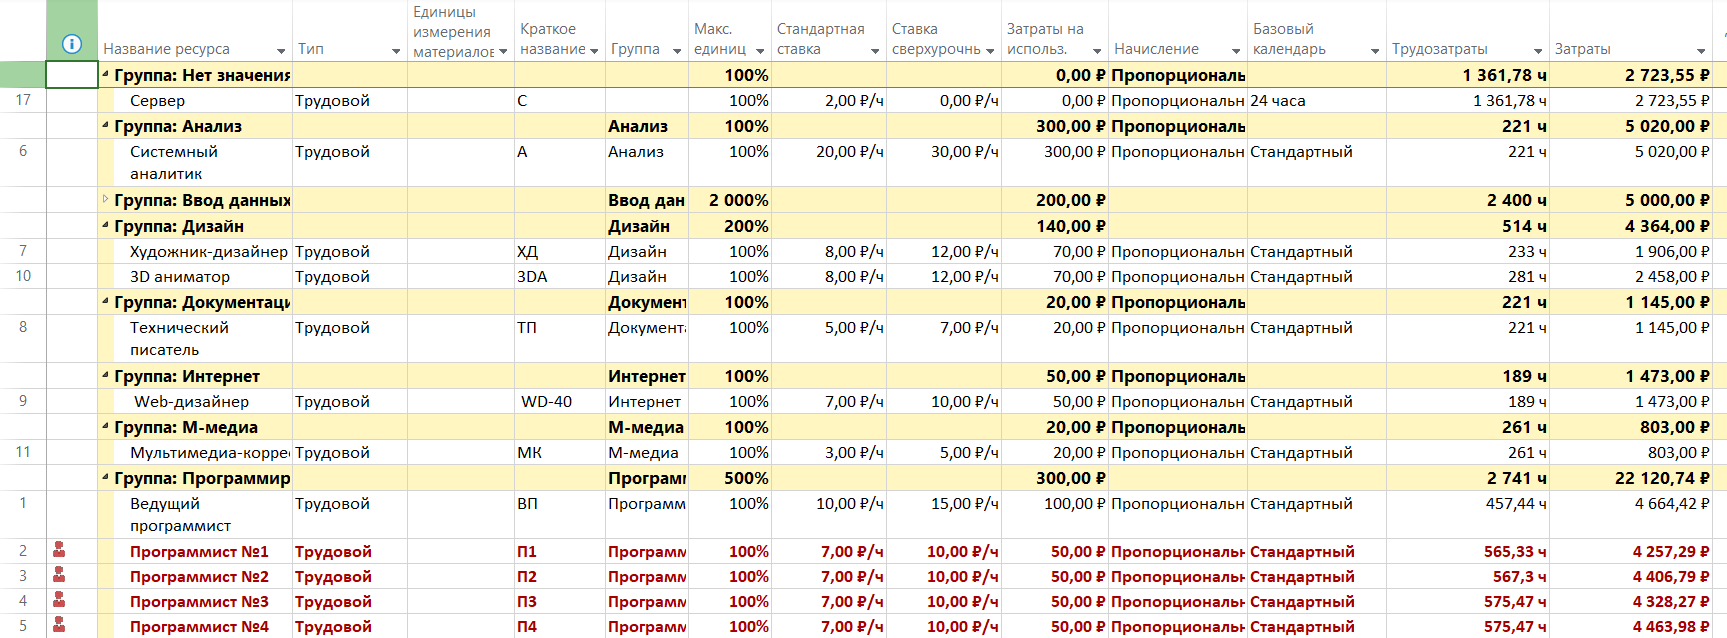
\includegraphics[width=\linewidth]{images/peregruz_komandirovka_resurs.png}
	\caption{Перегрузки, возникшие в результате отправки программистов №1 и №3 в командировку и увеличения длительности рабочего дня программистам №2 и №4}
	\label{fig:13}
\end{figure}

\begin{figure}[H]
	\centering
	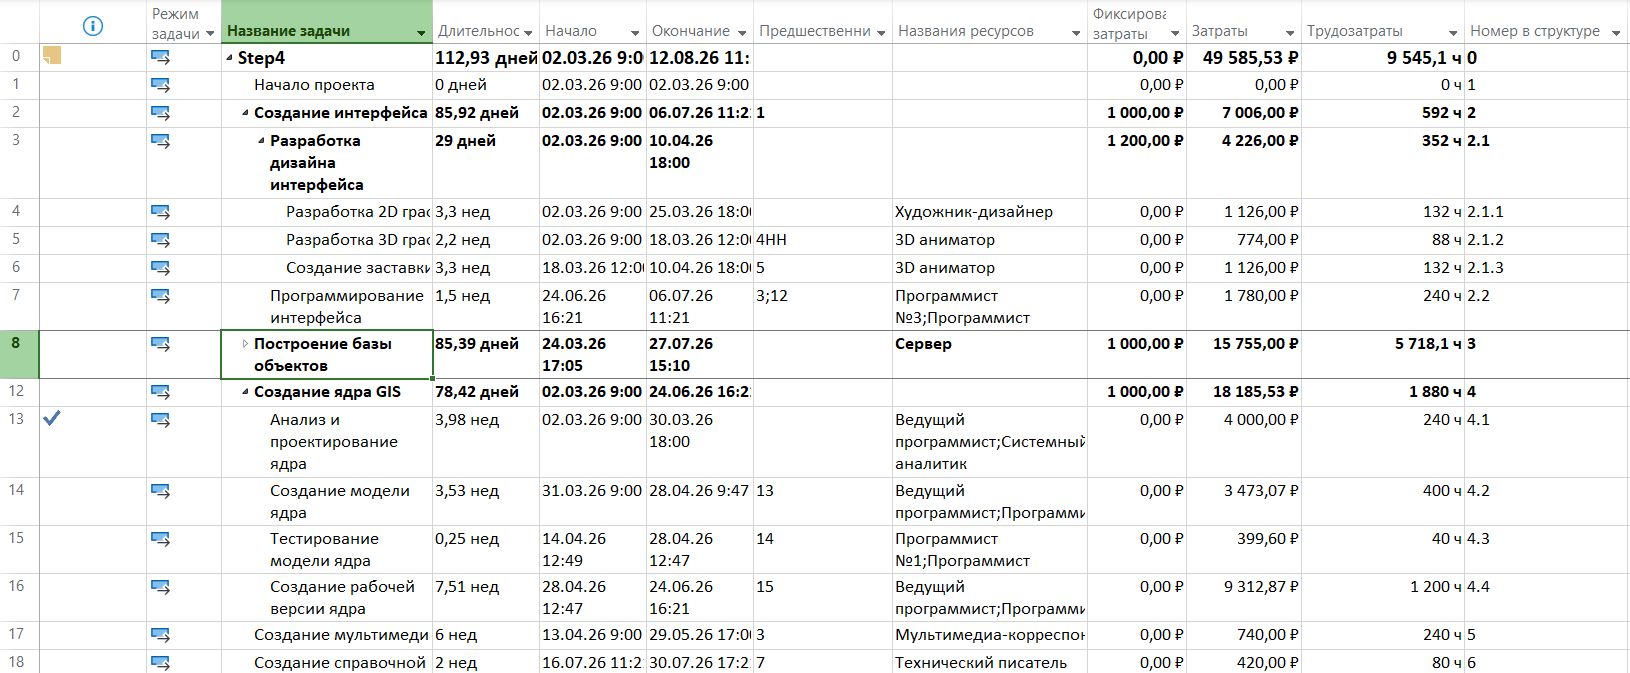
\includegraphics[width=\linewidth]{images/solve_peregruz_komandirovka_po_chasam_best.png}
	\caption{Результат разрешения перегрузки ресурсов}
	\label{fig:14}
\end{figure}

\section{Задание 5}

Для увольнения наборщика данных, необходимо изменить параметры его доступности, как показано на рисунке~\ref{fig:15}. В результате возникла перегрузка по задаче наполнения базы объектов ~\ref{fig:16}. В связи с тем, что задача начинается после увольнения сотрудника, данный сотрудник был попросту исключен из доступных ресурсов задачи. Данное действие привело к тому, что затраты возросли до 49 618,17 (+32,64) рублей, в связи с увеличением срока использования сервера. Сроки проекта при этом не изменились, так как данная задача не лежит на критическом пути~\ref{fig:17}.

\begin{figure}[H]
	\centering
	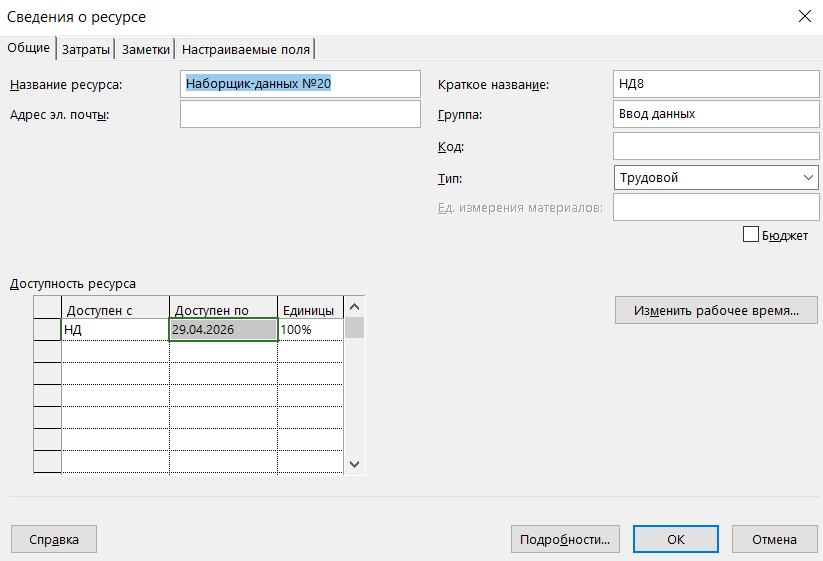
\includegraphics[width=0.7\linewidth]{images/uvolen.png}
	\caption{Изменений сведений о доступности сотрудника в связи с увольнением}
	\label{fig:15}
\end{figure}

\begin{figure}[H]
	\centering
	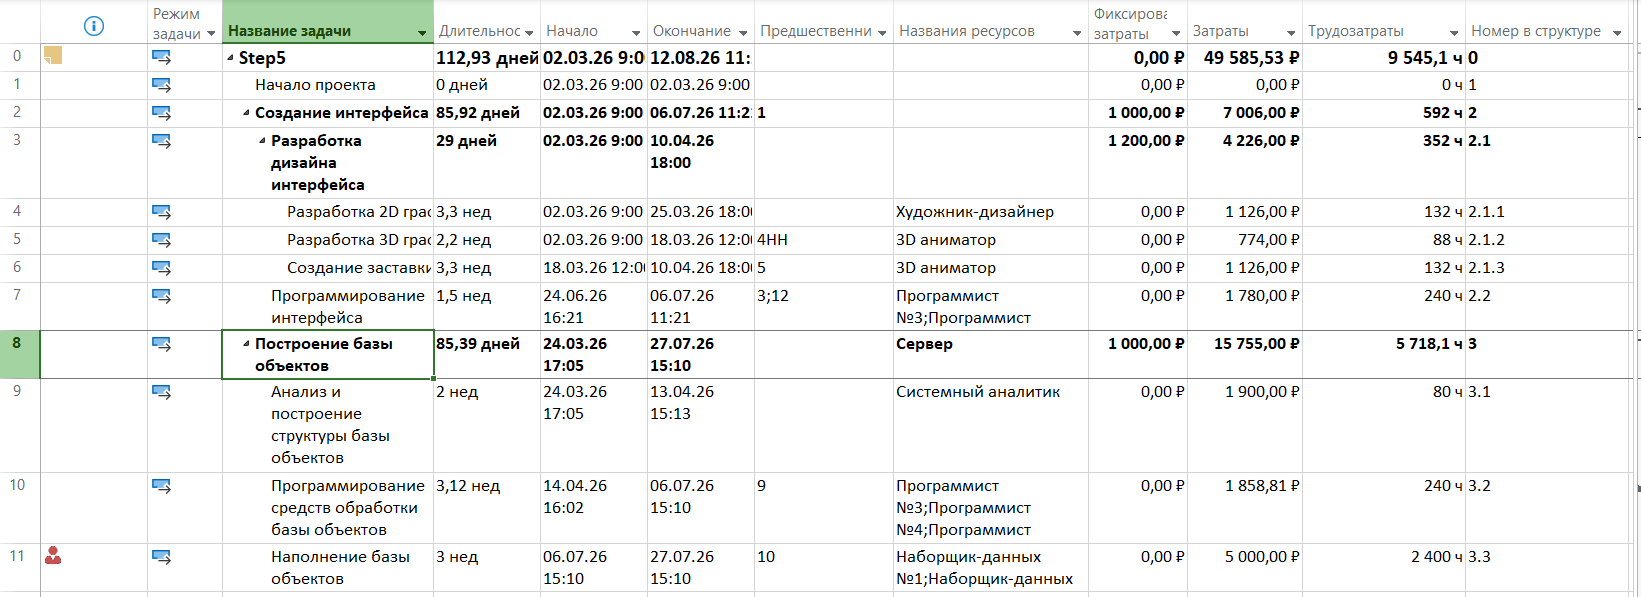
\includegraphics[width=\linewidth]{images/peregruz_uvolen.png}
	\caption{Перегрузка ресурсов в связи с увольнением сотрудника}
	\label{fig:16}
\end{figure}

\begin{figure}[H]
	\centering
	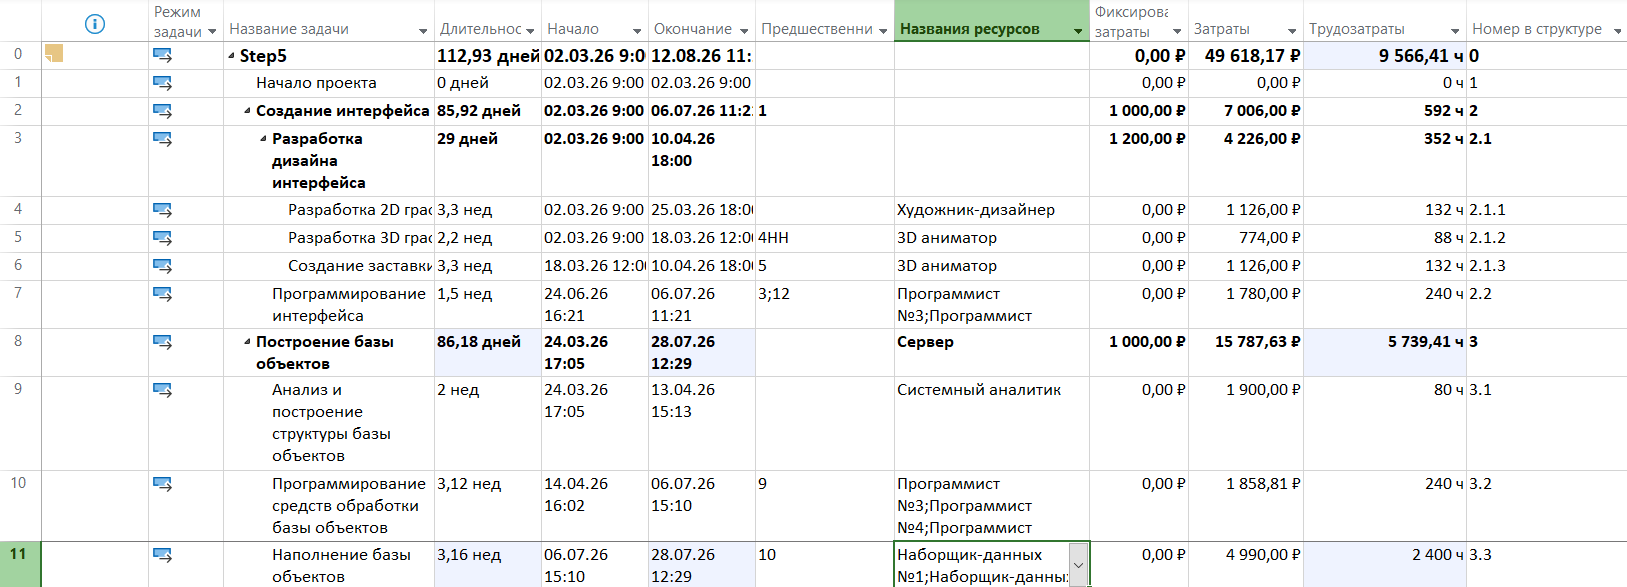
\includegraphics[width=\linewidth]{images/solve_peregruz_uvolen_nu_sebal_i_sebal_vse_ravno_do_starta_zadachi.png}
	\caption{Результат разрешения перегрузки по задаче наполнения базы объектов}
	\label{fig:17}
\end{figure}

\section{Задание 6}

Для отображения увеличения стоимости аренды сервера, был изменен план оплаты, как показано на рисунке~\ref{fig:18}. В результате затраты проекта выросли до
49 877,72 (+259,55) рублей~\ref{fig:19}
\begin{figure}[H]
	\centering
	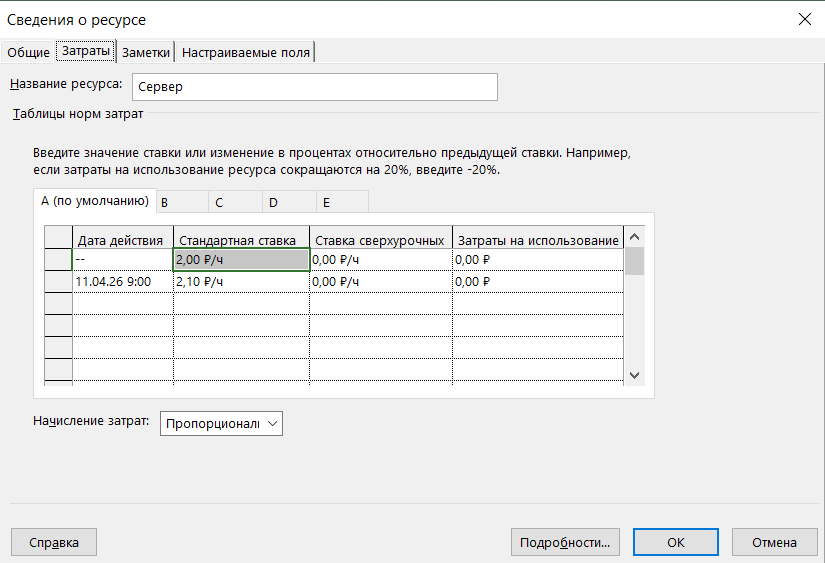
\includegraphics[width=0.7\linewidth]{images/server_babki.png}
	\caption{Изменение плана оплаты в связи с увеличением стоимости аренды сервера}
	\label{fig:18}
\end{figure}

\begin{figure}[H]
	\centering
	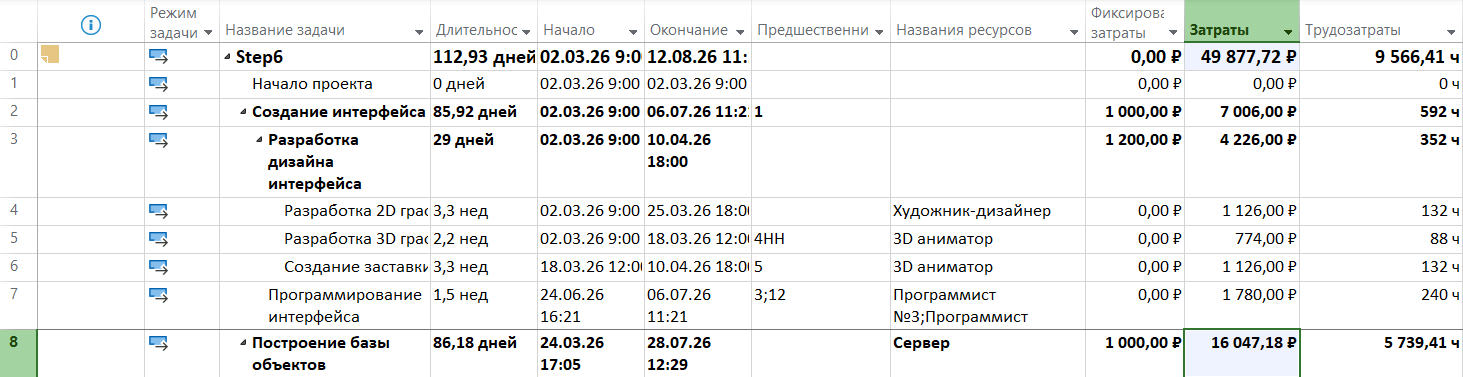
\includegraphics[width=\linewidth]{images/wasted_server.png}
	\caption{Изменение затрат проекта в связи с увеличением стоимости аренды сервера}
	\label{fig:19}
\end{figure}

\section*{Выводы}

В результате описанных изменений, сроки выполнения проекта сдвинулись на 21 день до 12.08, запас до максимально возможного срока составляет 20 дней. Затраты проекта также увеличились на 5077,76 рублей до 49 877,72 рублей. Запас финансов до максимально возможного бюджета составляет всего 122,28 рублей. Линия хода выполнения проекта представлена на рисунке~\ref{fig:20}.

\begin{figure}[H]
	\centering
	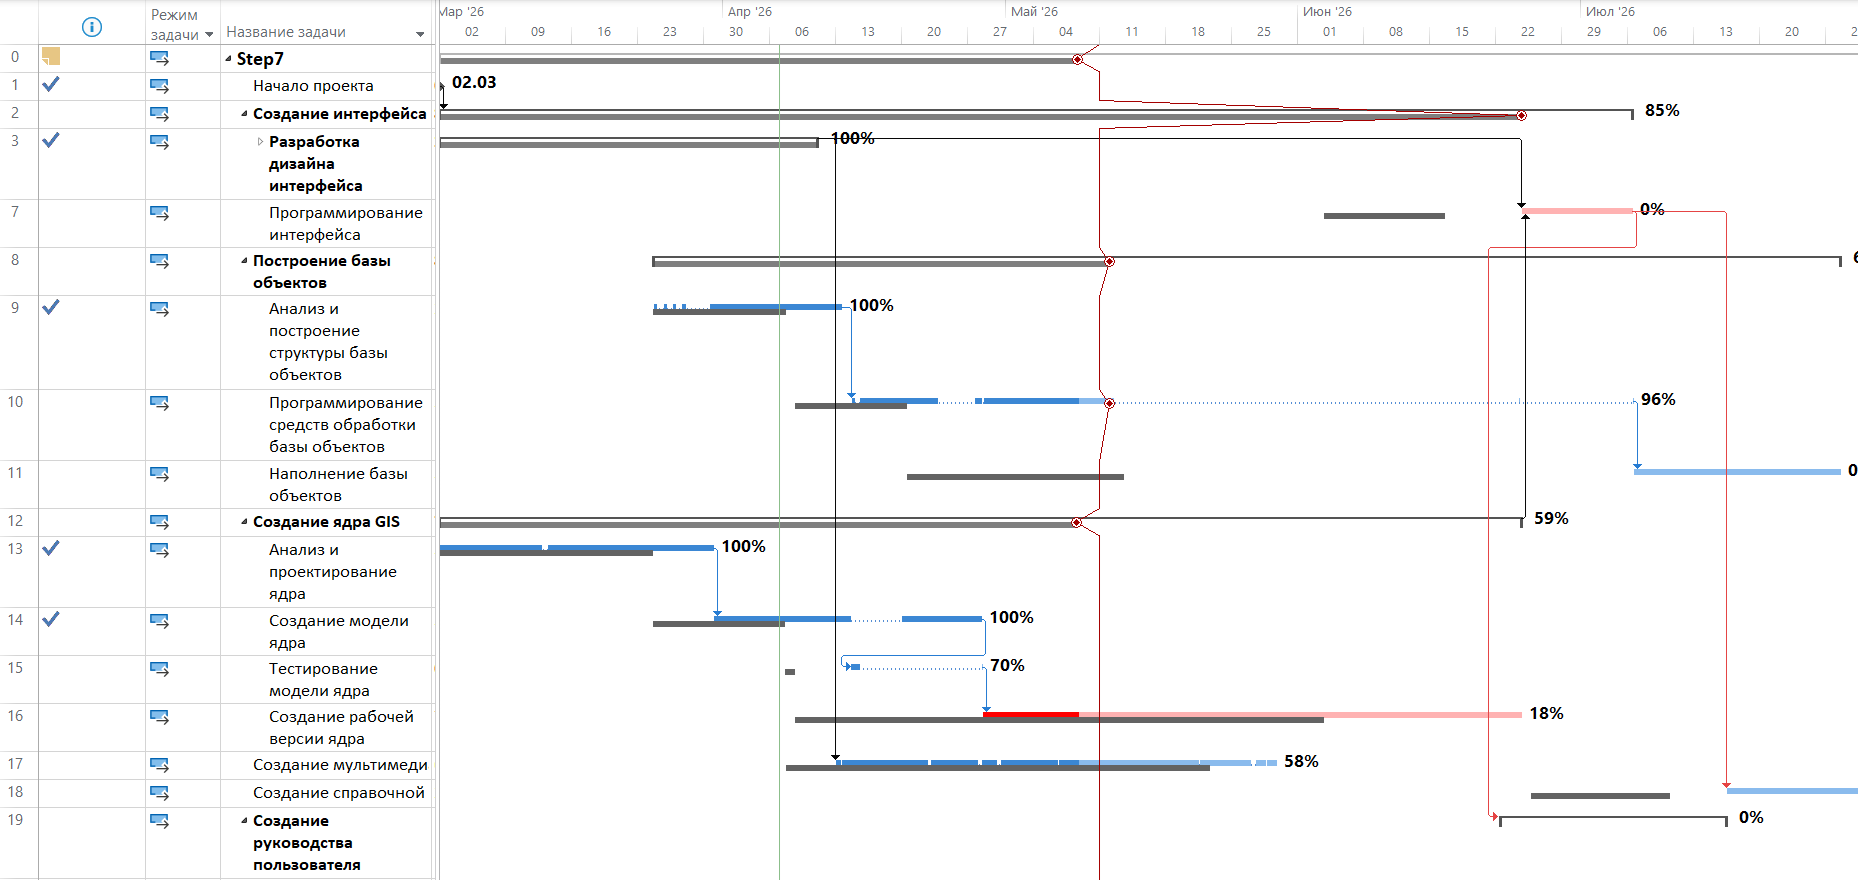
\includegraphics[width=\linewidth]{images/line.png}
	\caption{Линия хода выполнения проекта}
	\label{fig:20}
\end{figure}

Исходя из линии хода выполнения большинство работ идут по графику, несмотря на запаздывание отдельных работ, присутствует достаточный запас времени для завершения проекта до максимального срока.